\section{Sở GD \& ĐT Hà Nội, Cụm Đông lần 1, 25--26}
% ==============================================================================
% PHẦN I. CÂU TRẮC NGHIỆM NHIỀU PHƯƠNG ÁN LỰA CHỌN
% ==============================================================================
\caulc
\Opensolutionfile{ans}[ans/ans-22-26-2-HaNoi-CumDong-L1-LC]
\begin{ex}%[2H2H2-2]
    Trong không gian với hệ trục tọa độ $Oxyz$, cho ba điểm không thẳng hàng $A(-12;10;-2)$, $B(-4;6;9)$ và $E(6;-6;4)$. Để tứ giác $ABEF$ là hình bình hành thì tọa độ điểm $F$ là
    \choice
    {$(-14;10;-15)$}
    {$(-10;10;11)$}
    {$(-22;22;3)$}
    {\True $(-2;-2;-7)$}
    \loigiai{
        Tứ giác $ABFE$ là hình bình hành $\Leftrightarrow \overline{AB}=\overline{FE}$.\\
        Gọi điểm $F(a;b;c) \Rightarrow \overline{FE}=(6-a;-6-b;4-c)$ và $\overline{AB}=(8;-4;11)$.\\
        Ta có $\heva{&6-a=8\\& -6-b=-4\\& 4-c=11} \Leftrightarrow \heva{&a=-2\\& b=-2\\& c=-7} \Rightarrow F(-2;-2;-7)$.
    }
\end{ex}

\begin{ex}%[2D1H5-1]
\immini{Đồ thị hàm số phân thức bậc nhất trên bậc nhất nào dưới đây có hình vẽ như hình bên?
    \choice
    {$y=\dfrac{-x+2}{x+1}$}
    {$y=\dfrac{-x}{x+1}$}
    {\True $y=\dfrac{-x+1}{x+1}$}
    {$y=\dfrac{-2x+1}{2x+1}$}
	}{
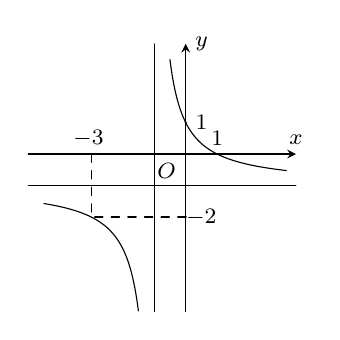
\begin{tikzpicture}[line join=round,line cap=round, font=\footnotesize,scale=0.4,>=stealth]
	\draw[-stealth](-5,0)--(3.5,0)node[above]{$x$};
	\draw[-stealth](0,-5)--(0,3.5)node[right]{$y$};		
	\draw[smooth,samples=300,domain=-0.5:3.2] plot(\x,{(-\x+1)/(\x+1)});
	\draw[smooth,samples=300,domain=-4.5:-1.5] plot(\x,{(-\x+1)/(\x+1)});	
	\fill (0,0) circle(1pt)node[below left]{$O$}; 				
	\foreach \x/\g in {-3/100,1/90}\fill[black] (\x,0) circle (1pt)+(\g:.5)node{$\x$};
		\foreach \x/\g in {-2/0,1/0}\fill[black] (0,\x) circle (1pt)+(\g:.5)node{$\x$};
		\draw (-1,-5)--(-1,3.5);
		\draw[domain=-5:3.5] plot(\x,-1);
		\draw[dashed] (-3,0)|-(0,-2);						
\end{tikzpicture}	
	}
    \loigiai{
        Đồ thị hàm số đã cho có tiệm cận đứng là $x=-1$, tiệm cận ngang là $y=-1$.\\
        Đồ thị đi qua điểm $A(1;0)$ và $B(0;1)$.\\
        Vậy hàm số cần tìm là $y=\dfrac{-x+1}{x+1}$.
    }
\end{ex}

\begin{ex}%[1D2H3-3]
    Công bội của cấp số nhân $(u_{n})$ biết $u_{3}=4$ và $u_{4}=8$ là
    \choice
    {$q=-4$}
    {\True $q=2$}
    {$q=\dfrac{1}{2}$}
    {$q=4$}
    \loigiai{
        Ta có $q=\dfrac{u_{4}}{u_{3}}=\dfrac{8}{4}=2$.
    }
\end{ex}

\begin{ex}%[1D6H4-3]
    Tập nghiệm của bất phương trình $\log_{0{,}5}(x-1)>1$ là
    \choice
    {$\left(-\infty;-\dfrac{3}{2}\right)$}
    {$\left(1;\dfrac{3}{2}\right)$}
    {\True $\left(1;\dfrac{3}{2}\right)$}
    {$\left(\dfrac{3}{2};+\infty\right)$}
    \loigiai{
        Ta có $\log_{0{,}5}(x-1)>1 \Leftrightarrow \heva{&x-1>0\\& x-1<0{,}5^{1}} \Leftrightarrow \heva{&x>1\\& x<\dfrac{3}{2}} \Leftrightarrow 1<x<\dfrac{3}{2}$.\\
        Vậy tập nghiệm của bất phương trình là $\left(1;\dfrac{3}{2}\right)$.
    }
\end{ex}

\begin{ex}%[2D1H3-1]
\immini{Cho hàm số $y=f(x)$ có đồ thị như hình vẽ. Hàm số đã cho đạt giá trị nhỏ nhất trên đoạn $[-1;1]$ tại
    \choice
    {\True $x=-1$}
    {$x=0$}
    {$x=-4$}
    {$x=1$}
	}{
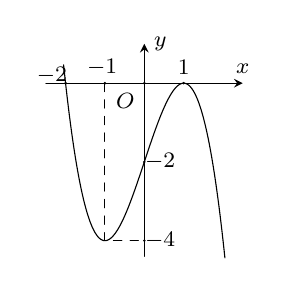
\begin{tikzpicture}[line join=round,line cap=round, font=\footnotesize,scale=0.5,>=stealth]
	\draw[-stealth](-2.5,0)--(2.5,0)node[above]{$x$};
	\draw[-stealth](0,-4.4)--(0,1)node[right]{$y$};		
	\draw[smooth,samples=300,domain=-2.05:2.05] plot(\x,{-(\x)^3+3*\x-2});	
	\fill (0,0) circle(1pt)node[below left]{$O$}; 				
	\foreach \x/\g in {-2/150,-1/100,1/90}\fill[black] (\x,0) circle (1pt)+(\g:.4)node{$\x$};
	\foreach \x/\g in {-4/0,-2/0}\fill[black] (0,\x) circle (1pt)+(\g:.4)node{$\x$};	
	\draw[dashed] (-1,0)|-(0,-4);						
\end{tikzpicture}	
	}
    \loigiai{
        Dựa vào đồ thị hàm số $y=f(x)$, ta thấy hàm số đồng biến trên đoạn $[-1;1]$ nên hàm số đạt giá trị nhỏ nhất trên đoạn $[-1;1]$ tại $x=-1$.
    }
\end{ex}

\begin{ex}%[1H8H6-2]
    Cho hình chóp $S.ABC$ có $SA\perp(ABC)$, $SA=\dfrac{3a}{2}$ và đáy $ABC$ là tam giác đều cạnh $a$. Tính số đo của góc nhị diện $[S,BC,A]$.
    \choice
    {$30^{\circ}$}
    {$90^{\circ}$}
    {$120^{\circ}$}
    {\True $60^{\circ}$}
    \loigiai{
\immini{Gọi $M$ là trung điểm của $BC$.\\
        Ta có $\heva{&BC\perp AM\\& BC\perp SA} \Rightarrow BC\perp(SAM) \Rightarrow BC\perp SM$.\\
        Khi đó góc nhị diện $[S,BC,A] = \widehat{SMA}$.\\
        Xét tam giác $SAM$ vuông tại $A$, ta có\\
        $\tan \widehat{SMA}=\dfrac{SA}{AM}=\dfrac{\dfrac{3a}{2}}{\dfrac{a\sqrt{3}}{2}}=\sqrt{3} \Rightarrow \widehat{SMA}=60^{\circ}$.
        }{
\begin{tikzpicture}[scale=1, font=\footnotesize, line join=round, line cap=round, >=stealth]
	\def\a{3}
	\path
	(0,0) coordinate (A)
	(0:\a) coordinate (C)
	(-40:0.6*\a) coordinate (B)
	(90:0.9*\a) coordinate (S)		
	($(B)!0.5!(C)$) coordinate (M)			
	;
	\draw  (S)--(A)--(B)--(C)--(S)--(B)(S)--(M);
	\draw[dashed] (M)--(A)--(C);	
	\foreach \x/\g in {A/170,B/-90,C/0,M/-30,S/90}\fill[black] (\x) circle (1pt)+(\g:.3)node{$\x$};
\end{tikzpicture}
   }
    }
\end{ex}

\begin{ex}%[2D1H4-1]
    Cho hàm số $y=f(x)$ có bảng biến thiên như hình vẽ.
 	\begin{center}

\begin{tikzpicture}
\tkzTabInit[nocadre=false,lgt=1.2,espcl=2.5,deltacl=0.6]
{$x$ /0.8, $y'$ /0.8, $y$ /2}
{$-\infty$,$1$,$3$,$+\infty$}
\tkzTabLine {,+,d,+,z,-,}
\tkzTabVar {-/$-1$,+D-/$+\infty$/$-\infty$,+/$2$,-/$-\infty$}
\end{tikzpicture}
\end{center}   
Tính tổng số đường tiệm cận đứng và ngang.
    \choice
    {\True $2$}
    {$0$}
    {$1$}
    {$3$}
    \loigiai{
        Ta có $\lim\limits_{x\rightarrow 1^{-}}f(x)=+\infty \Rightarrow$ đồ thị hàm số có một đường tiệm cận đứng là $x=1$.\\
        Lại có $\lim\limits_{x\rightarrow -\infty}f(x)=-1 \Rightarrow$ đồ thị hàm số có một đường tiệm cận ngang là $y=-1$.\\
        Mặt khác $\lim\limits_{x\rightarrow +\infty}f(x)=-\infty$ nên không có tiệm cận ngang khi $x \to +\infty$.\\
        Vậy đồ thị hàm số có tổng số đường tiệm cận đứng và ngang là $2$.
    }
\end{ex}

\begin{ex}%[1D9H1-3]
    Hai khẩu pháo cao xạ cùng bắn độc lập vào một mục tiêu. Xác suất bắn trúng mục tiêu của hai khẩu pháo cao xạ lần lượt là $\dfrac{1}{4}$ và $\dfrac{1}{3}$. Xác suất để mục tiêu bị trúng đạn là
    \choice
    {\True $\dfrac{1}{2}$}
    {$\dfrac{7}{12}$}
    {$\dfrac{5}{12}$}
    {$\dfrac{1}{4}$}
    \loigiai{
        Gọi biến cố $A_{1}$: \lq\lq Khẩu pháo thứ nhất bắn trúng\rq\rq, $\mathrm{P}\left(A_{1}\right)=\dfrac{1}{4} \Rightarrow \mathrm{P}\left(\overline{A}_{1}\right)=\dfrac{3}{4}$.\\
        Biến cố $A_{2}$: \lq\lq Khẩu pháo thứ hai bắn trúng\rq\rq, $\mathrm{P}\left(A_{2}\right)=\dfrac{1}{3} \Rightarrow \mathrm{P}\left(\overline{A}_{2}\right)=\dfrac{2}{3}$.\\
        Biến cố $\overline{A}$: \lq\lq Mục tiêu không bị trúng đạn\rq\rq.\\
        Vì $A_{1}$, $A_{2}$ độc lập nên $\mathrm{P}\left(\overline{A}\right)=\mathrm{P}\left(\overline{A}_{1}\right) \cdot \mathrm{P}\left(\overline{A}_{2}\right) = \dfrac{3}{4} \cdot \dfrac{2}{3} = \dfrac{1}{2}$.\\
        Vậy xác suất để mục tiêu bị trúng đạn là $\mathrm{P}(A)=1-\mathrm{P}\left(\overline{A}\right)=1-\dfrac{1}{2}=\dfrac{1}{2}$.
    }
\end{ex}

\begin{ex}%[1D1H5-3]
    Phương trình $\sin x=-1$ có nghiệm là
    \choice
    {$x=\dfrac{\pi}{2}+k2\pi$, $k\in\mathbb{Z}$}
    {$x=\pi+k2\pi$, $k\in\mathbb{Z}$}
    {$x=k\pi$, $k\in\mathbb{Z}$}
    {\True $x=-\dfrac{\pi}{2}+k2\pi$, $k\in\mathbb{Z}$}
    \loigiai{
        Ta có công thức nghiệm cơ bản $\sin x=-1 \Leftrightarrow x=-\dfrac{\pi}{2}+k2\pi$, $k\in\mathbb{Z}$.
    }
\end{ex}

\begin{ex}%[1D5H1-3]
    Khảo sát thu nhập theo tháng của người lao động ở một công ty thu được mẫu số liệu ghép nhóm như sau
    \begin{center}
    \begin{tabular}{|c|c|c|c|c|c|}
    \hline
    Thu nhập (triệu đồng) & $[5;8)$ & $[8;11)$ & $[11;14)$ & $[14;17)$ & $[17;20)$ \\ \hline
    Số người & $30$ & $55$ & $45$ & $30$ & $20$ \\ \hline
    \end{tabular}
    \end{center}
    Tính mức thu nhập trung bình của người lao động ở công ty trên (đơn vị: triệu đồng).
    \choice
    {$10{,}5$}
    {\True $11{,}75$}
    {$12{,}5$}
    {$11$}
    \loigiai{
        Giá trị đại diện của các nhóm lần lượt là $x_1=6{,}5$; $x_2=9{,}5$; $x_3=12{,}5$; $x_4=15{,}5$; $x_5=18{,}5$.\\
        Mức thu nhập trung bình là    
   $$\overline{x}=\dfrac{6{,}5 \cdot 30 + 9{,}5 \cdot 55 + 12{,}5 \cdot 45 + 15{,}5 \cdot 30 + 18{,}5 \cdot 20}{30+55+45+30+20}=\dfrac{2115}{180}=11{,}75 \text{ (triệu đồng)}.$$ 
    }
\end{ex}

\begin{ex}%[2D1H2-2]
	\immini{
    Cho hàm số $y=f(x)$ có bảng biến thiên như sau.
     Hàm số $y=f(x)$ đạt cực tiểu tại điểm:
    \choice
    {$y=0$}
    {$x=-4$}
    {$y=4$}
    {\True $x=3$}
    }{
    
\begin{tikzpicture}
    	\tkzTabInit[nocadre=false,lgt=1.2,espcl=1.8,deltacl=0.6]
    	{$x$ /0.6, $f'(x)$ /0.6, $f(x)$ /2}
    	{$-\infty$,$0$,$3$,$+\infty$}
    	\tkzTabLine {,+,z,-,z,+,}
    	\tkzTabVar {-/$-\infty$,+/$2$,-/$4$,+/$+\infty$}
    \end{tikzpicture}
    }
    \loigiai{
        Dựa vào bảng biến thiên, ta thấy đạo hàm $f'(x)$ đổi dấu từ âm sang dương khi qua điểm $x=3$. Do đó, hàm số đạt cực tiểu tại điểm $x=3$.
    }
\end{ex}

\begin{ex}%[2H2H2-2]
    Trong không gian $Oxyz$, cho điểm $A(1;0;1)$. Tìm tọa độ điểm $C$ thỏa mãn $\overline{AC}=(3;3;0)$?
    \choice
    {$C(2;3;1)$}
    {$C(3;3;0)$}
    {$C(-3;-3;-1)$}
    {\True $C(4;3;1)$}
    \loigiai{
        Giả sử điểm $C(x;y;z)$, ta có $\overline{AC}=(x-1;y;z-1)$.\\
        Theo giả thiết $\overline{AC}=(3;3;0) \Leftrightarrow \heva{&x-1=3\\& y=3\\& z-1=0} \Leftrightarrow \heva{&x=4\\& y=3\\& z=1} \Rightarrow C(4;3;1)$.
    }
\end{ex}
\Closesolutionfile{ans}
% ==============================================================================
% PHẦN II. CÂU TRẮC NGHIỆM ĐÚNG SAI
% ==============================================================================
\cauds
\Opensolutionfile{ans}[ans/ans-22-26-2-HaNoi-CumDong-L1-DS]
\begin{ex}%[1H8V7-3]
    Cho hình vuông $ABCD$ có cạnh bằng $4$. Lấy $H$, $K$ lần lượt trên các cạnh $AB$, $AD$ sao cho $BH=3HA$, $AK=3KD$. Trên đường thẳng vuông góc với mặt phẳng $(ABCD)$ tại $H$ lấy điểm $S$ sao cho $\widehat{SBH}=30^{\circ}$. Xét tính đúng sai của các khẳng định sau:
    \choiceTF
    {\True Thể tích của khối chóp $S.ABCD$ bằng $\dfrac{16\sqrt{3}}{3}$}
    {\True Khoảng cách giữa $AB$ và $SD$ bằng $\dfrac{4\sqrt{57}}{19}$}
    {\True $SH = \sqrt{3}$}
    {\True Gọi $E$ là giao điểm của $CH$ và $BK$, cosin của góc giữa hai đường thẳng $SE$ và $BC$ bằng $\dfrac{m}{n\sqrt{39}}$, với $m\in\mathbb{Z}$, $n\in\mathbb{N}^*$, $\dfrac{m}{n}$ là phân số tối giản. Giá trị của biểu thức $T=2m-n=31$}
    \loigiai{
    \begin{center}
    \begin{tikzpicture}[scale=1, font=\footnotesize, line join=round, line cap=round, >=stealth]
	\def\a{3}
	\path
	(0,0) coordinate (A)
	(0:\a) coordinate (B)
	(220:0.6*\a) coordinate (D)	
	($(B)+(D)$) coordinate (C)
	($(A)!0.25!(B)$) coordinate (H)
	($(H)!1.4!90:(B)$) coordinate (S)
	($(A)!0.75!(D)$) coordinate (K)
	(intersection of C--H and B--K) coordinate (E)
	($(D)!0.25!(C)$) coordinate (M)
	($(B)!0.65!(H)$) coordinate (G)
	($(S)!0.6!(M)$) coordinate (I)			
	;
	\draw  (S)--(B)--(C)--(D)--(S)--(C)(S)--(M);
	\draw[dashed] (D)--(A)--(B) (S)--(A)(C)--(H)(S)--(H)(B)--(K)(H)--(M)(E)--(G)(H)--(I)(S)--(G)(S)--(E);	
	\foreach \x/\g in {A/-100,B/0,C/-30,D/180,S/90,H/-90,K/70,E/-90,M/-90,G/40,I/200}\fill[black] (\x) circle (1pt)+(\g:.3)node{$\x$};
\end{tikzpicture}
    \end{center}
Ta có $HB=3$, $SH \perp (ABCD)$, $\widehat{SBH}=30^{\circ} \Rightarrow SH = HB \cdot \tan 30^{\circ} = 3 \cdot \dfrac{\sqrt{3}}{3} = \sqrt{3}$.
	\begin{itemchoice}
	\itemch $V_{S.ABCD} = \dfrac{1}{3} \cdot SH \cdot S_{ABCD} = \dfrac{1}{3} \cdot \sqrt{3} \cdot 4^2 = \dfrac{16\sqrt{3}}{3}$.\\
	\itemch Do $AB \parallel CD \Rightarrow AB \parallel (SCD) \Rightarrow \mathrm{d}(AB, SD) = \mathrm{d}(H, (SCD))$.\\
	 Kẻ $HM \perp CD \Rightarrow MC=3MD$; $HM = 4$.\\
	 Kẻ $HI \perp SM\quad(1)$\\
	 Khi đó $\heva{&CD\perp HM\\&CD\perp SH}\Rightarrow CD\perp SHM\Rightarrow CD\perp HI\quad (2)$\\
	 Từ $(1)$ và $(2)$ suy ra $HI\perp (SCD)$ nên $HI=\mathrm{d}(H,(SCD))$.\\
	 Trong tam giác vuông $SHM$ ta có\\
	  $HI = \dfrac{SH \cdot HM}{\sqrt{SH^2+HM^2}} = \dfrac{\sqrt{3} \cdot 4}{\sqrt{3+16}} = \dfrac{4\sqrt{57}}{19}$.
	\itemch Ta có $SH = \sqrt{3}$.
	\itemch Ta có $\triangle ABK=\triangle BCH\Rightarrow \widehat{ABK}=\widehat{BCH}$.\\
Mà $\widehat{ABK}+\widehat{KBC}=90^\circ\Rightarrow \widehat{EBC}+\widehat{ECB}=90^\circ$, hay $BK\perp CH$ tại $E$.\\
Trong tam giác vuông $BCH$, có đường cao $BE$, suy ra\\
 $BE=\dfrac{BH\cdot BC}{HC}=\dfrac{3\cdot4}{\sqrt{3^2+4^2}}=2{,}4$;
$HE=\dfrac{BH^2}{HC}=1{,}8$.\\
Kẻ $EG\perp AB\Rightarrow EG\parallel BC\Rightarrow(SE;BC)=(SE;EG)=\widehat{SEG}$.\\
Ta có $GE=\dfrac{BE\cdot HE}{BH}=1{,}44\Rightarrow HG^2=HE^2-GE^2=\dfrac{729}{625}$.\\
Trong tam giác vuông $SHG$ có $SG^2=SH^2+HG^2=3+\dfrac{729}{625}=\dfrac{2604}{625}$.\\
Trong tam giác vuông $SHE$ có $SE=\sqrt{SH^2+HE^2}=\sqrt{3+(1{,}8)^2}=\dfrac{2\sqrt{39}}{5}$.\\
Áp dụng định lý cosin trong tam giác $SGE$ có\\
$\cos(\widehat{SEG})=\dfrac{SE^2+GE^2-SG^2}{2\cdot SE\cdot GE}=\dfrac{18}{5\sqrt{39}}\Rightarrow m=18,n=5$.\\
Suy ra $T=2m-n=31$.
	\end{itemchoice}
    }
\end{ex}

\begin{ex}%[2H2V2-6]
    Trong không gian, xét hệ tọa độ $Oxyz$ có gốc trùng với vị trí một giàn khoan trên biển, mặt phẳng $(Oxy)$ trùng với mặt biển với tia $Ox$ hướng về phía nam, tia $Oy$ hướng về phía đông, tia $Oz$ hướng thẳng lên trời. Đơn vị đo lấy theo kilômét. Một chiếc radar đặt tại $O$ có phạm vi theo dõi $30$ km. Một chiếc tàu thám hiểm tại vị trí $A$ có độ sâu $10$ km so với mặt nước biển, cách $O$ $25$ km về phía nam và $15$ km về phía tây. Một tàu đánh cá tại vị trí $B(-20;15;0)$. Xét tính đúng sai của các khẳng định sau:
    \choiceTF
    {\True Một chiếc tàu của cảnh sát biển đang di chuyển đến vị trí $C$ cách $O$ $15$ km về phía nam. Để trong phạm vi theo dõi của radar thì tàu cảnh sát biển cần di chuyển về phía đông cách $O$ tối đa $15\sqrt{3}$ km}
    {\True Radar phát hiện ra tàu đánh cá tại vị trí $B$}
    {Khoảng cách từ chiếc tàu thám hiểm đến radar bằng $3\sqrt{58}$ km}
    {\True Radar không phát hiện được tàu thám hiểm đặt tại vị trí $A$}
    \loigiai{
        Phạm vi radar là bán kính $R = 30$ km. Từ giả thiết ta có hệ trục: $Ox$ hướng Nam, $Oy$ hướng Đông, $Oz$ hướng lên trời.
	\begin{itemchoice}
	\itemch Một chiếc tàu của cảnh sát biển đang tuần tra trên biển di chuyển đến vị trí $C$ cách $O$ $15$ km về phía nam. Do đó $C(15;y;0)$.\\
Suy ra $\overrightarrow{OC}=(15;y;0)\Rightarrow OC=\sqrt{15^2+y^2}$\\
Để tàu cảnh sát biển trong phạm vi theo dõi của radar thì $OC\le\mathbb{R}$, khi đó
\begin{align*}
\sqrt{15^2+y^2}\le30\Leftrightarrow y^2\le900-225\Leftrightarrow y^2\le675\Rightarrow|y|\le15\sqrt{3}.
\end{align*}
Vậy tàu cảnh sát biển cần di chuyển về phía đông cách $O$ tối đa $15\sqrt{3}$ km	\itemch Một tàu đánh cá tại vị trí $B(-20;15;0)$.\\
Suy ra $\overrightarrow{OB}=(-20;15;0)\Rightarrow OB=\sqrt{(-20)^2+15^2+0^2}=25<30$\\
Vậy radar phát hiện ra tàu đánh cá tại vị trí $B$.
	\itemch Tàu thám hiểm tại vị trí $A$ có độ sâu $10$ km so với mặt nước biển, cách $O$ $25$ km về phía nam và $15$ km về phía tây. Do đó $A(25;-15;-10)$\\
Suy ra $\overrightarrow{OA}=(25;-15;-10)\Rightarrow OA=\sqrt{(25)^2+(-15)^2+(-10)^2}=5\sqrt{38}$
	\itemch $\overrightarrow{OA}=(25;-15;-10)\Rightarrow OA=\sqrt{(25)^2+(-15)^2+(-10)^2}=5\sqrt{38}\approx30{,}8>30$.
	\end{itemchoice}
    }
\end{ex}

\begin{ex}%[2D1V5-7]
    Cho hàm số $y = f(x) = \dfrac{2x^2 - 5x + 9}{x - 5}$.
    \choiceTF
    {\True Đồ thị hàm số cắt trục tung tại điểm có tung độ bằng $-\dfrac{9}{5}$}
    {Hàm số nghịch biến trên khoảng $(1;9)$}
    {Có đúng một điểm trên đồ thị hàm số cách đều hai trục tọa độ}
    {Đồ thị hàm số có đường tiệm cận đứng là $y = 5$}
    \loigiai{
	\begin{itemchoice}
	\itemch Đồ thị hàm số cắt trục tung tại điểm có tung độ là $f(0)=-\dfrac{9}{5}$.
	\itemch Vì hàm số không xác định tại điểm $x = 5$.
	\itemch Giả sử điểm $M$ trên đồ thị có tọa độ là $M\left(x;\dfrac{2x^2-5x+9}{x-5}\right)$ với $x\ne5$.\\
Điểm $M$ cách đều hai trục tọa độ nghĩa là
\allowdisplaybreaks
\begin{eqnarray*}
&&|x|=\left|\dfrac{2x^2-5x+9}{x-5}\right|\Leftrightarrow|x^2-5x|=|2x^2-5x+9|\\
&\Leftrightarrow&\hoac{&x^2-5x=2x^2-5x+9\\&x^2-5x=-2x^2+5x-9}\Leftrightarrow\hoac{&x^2+9=0\\&3x^2-10x+9=0}\Leftrightarrow x\in\varnothing.
\end{eqnarray*}
Vậy không có điểm nào thỏa mãn.
	\itemch Đồ thị hàm số có đường tiệm cận đứng là $x = 5$.
	\end{itemchoice}
    }
\end{ex}

\begin{ex}%[1D1V5-3]
    Cho phương trình $\cos\left(4x - \dfrac{3\pi}{8}\right) = -1$. 
    \choiceTF
    {\True $x = \dfrac{11\pi}{32}$ là một nghiệm của phương trình đã cho}
    {\True Tất cả nghiệm của phương trình đã cho được biểu diễn bởi $4$ điểm trên đường tròn lượng giác}
    {Tổng nghiệm dương nhỏ nhất và nghiệm âm lớn nhất của phương trình bằng $\dfrac{3\pi}{4}$}
    {Tổng các nghiệm trên khoảng $\left(\dfrac{\pi}{4}; \dfrac{19\pi}{2}\right)$ của phương trình đã cho là $\dfrac{6061\pi}{32}$}
    \loigiai{
	\begin{itemchoice}
	\itemch Thay $x=\dfrac{11\pi}{32}$ vào phương trình, ta được: $\cos\left(4\cdot\dfrac{11\pi}{32}-\dfrac{3\pi}{8}\right)=\cos(\pi)=-1$.\\
Vậy $x=\dfrac{11\pi}{32}$ là một nghiệm của phương trình đã cho.
	\itemch Ta có\\
$\cos\left(4x-\dfrac{3\pi}{8}\right)=-1\Leftrightarrow4x-\dfrac{3\pi}{8}=\pi+k2\pi\Leftrightarrow4x=\dfrac{11\pi}{8}+k2\pi\Leftrightarrow x=\dfrac{11\pi}{32}+\dfrac{k\pi}{2}(k\in\mathbb{Z})$.\\
Áp dụng công thức nghiệm $x=\alpha+\dfrac{k2\pi}{n}$ với $n$ là số điểm biểu diễn trên đường tròn lượng giác, ta có\\
 $\Leftrightarrow x=\dfrac{11\pi}{32}+\dfrac{k\pi}{2}=\dfrac{11\pi}{32}+\dfrac{k2\pi}{4}$. Suy ra $n=4$.\\
Vậy tất cả nghiệm của phương trình đã cho được biểu diễn bởi $4$ điểm trên đường tròn lượng giác.
	\itemch Xét $x=\dfrac{11\pi}{32}+\dfrac{k\pi}{2}>0\Leftrightarrow\dfrac{k\pi}{2}>-\dfrac{11\pi}{32}\Leftrightarrow k>-\dfrac{11}{16}$ mà $k\in\mathbb{Z}$.\\
Suy ra nghiệm dương nhỏ nhất ứng với $k=0$.\\
Nghiệm dương nhỏ nhất là $\dfrac{11\pi}{32}+\dfrac{0\cdot\pi}{2}=\dfrac{11\pi}{32}$.\\
Xét $x=\dfrac{11\pi}{32}+\dfrac{k\pi}{2}<0\Leftrightarrow\dfrac{k\pi}{2}<-\dfrac{11\pi}{32}\Leftrightarrow k<-\dfrac{11}{16}$ mà $k\in\mathbb{Z}$.\\
Suy ra nghiệm âm lớn nhất ứng với $k=-1$.\\
Nghiệm âm lớn nhất là $\dfrac{11\pi}{32}+\dfrac{(-1)\cdot\pi}{2}=-\dfrac{5\pi}{32}$.\\
Tổng nghiệm dương nhỏ nhất và nghiệm âm lớn nhất của phương trình bằng 
\begin{align*}
\dfrac{11\pi}{32}-\dfrac{5\pi}{32}=\dfrac{3\pi}{16}.
\end{align*}
	\itemch Do 
\allowdisplaybreaks
\begin{eqnarray*}	
&&x\in\left(\dfrac{\pi}{4};\dfrac{19\pi}{2}\right)\Leftrightarrow\dfrac{\pi}{4}<x<\dfrac{19\pi}{2}\Leftrightarrow\dfrac{\pi}{4}<\dfrac{11\pi}{32}+\dfrac{k\pi}{2}<\dfrac{19\pi}{2}\Leftrightarrow\dfrac{1}{4}<\dfrac{11}{32}+\dfrac{k}{2}<\dfrac{19}{2}\\
&\Leftrightarrow&-\dfrac{3}{32}<\dfrac{k}{2}<\dfrac{293}{32}\Leftrightarrow-\dfrac{3}{16}<k<\dfrac{293}{16},k\in\mathbb{Z}\Leftrightarrow k\in\{0;1;2;\dots;17;18\}.\\
\end{eqnarray*}
Thay các giá trị của $k$ vào $x=\dfrac{11\pi}{32}+\dfrac{k\pi}{2}$ ta được tập hợp các nghiệm trên khoảng $\left(\dfrac{\pi}{4};\dfrac{19\pi}{2}\right)$
\begin{align*}
x\in\left\{\dfrac{11\pi}{32};\dfrac{11\pi}{32}+\dfrac{\pi}{2};\dfrac{11\pi}{32}+\dfrac{2\pi}{2};\dots;\dfrac{11\pi}{32}+\dfrac{17\pi}{2};\dfrac{11\pi}{32}+\dfrac{18\pi}{2}\right\}.
\end{align*}
Tính tổng các nghiệm có $2$ cách:\\
\textbf{Cách 1:} Bấm máy $\sum\limits_{k=0}^{18}\left(\dfrac{11\pi}{32}+\dfrac{k\pi}{2}\right)=\dfrac{2945\pi}{32}$.\\
\textbf{Cách 2:} Tính: $\dfrac{11\pi}{32}+\left(\dfrac{11\pi}{32}+\dfrac{\pi}{2}\right)+\left(\dfrac{11\pi}{32}+\dfrac{2\pi}{2}\right)+\dots+\left(\dfrac{11\pi}{32}+\dfrac{17\pi}{2}\right)+\left(\dfrac{11\pi}{32}+\dfrac{18\pi}{2}\right)$.\\
Coi mỗi nghiệm là 1 số hạng trong cấp số cộng với $x_1=\dfrac{11\pi}{32}$, công sai $d=\dfrac{\pi}{2}$.\\
Do $k\in\{0;1;2;\dots;17;18\}$ nên số số hạng $n=19$.\\
Tổng các nghiệm là $S=\dfrac{(x_1+x_{19})\cdot n}{2}=\dfrac{\left(\dfrac{11\pi}{32}+\dfrac{11\pi}{32}+\dfrac{18\pi}{2}\right)\cdot19}{2}=\dfrac{2945\pi}{32}$.
	\end{itemchoice}
    }
\end{ex}

\Closesolutionfile{ans}

% ==============================================================================
% PHẦN III. CÂU TRẮC NGHIỆM TRẢ LỜI NGẮN
% ==============================================================================
\caukq
\Opensolutionfile{ans}[ans/ans-22-26-2-HaNoi-CumDong-L1-KQ]
\begin{ex}%[1H8V5-4]
    Cho hình chóp $S.ABCD$ có đáy $ABCD$ là hình thoi cạnh bằng $1$ đơn vị, $\widehat{BAD}=60^{\circ}$. Tam giác $SAB$ vuông cân tại $S$ và nằm trong mặt phẳng vuông góc với đáy. Biết khoảng cách từ $AB$ đến $SC$ bằng $\dfrac{\sqrt{a}}{b}$ ($a, b \in \mathbb{Z}^+$, $\dfrac{a}{b}$ là phân số tối giản). Tính tổng $a+b$.\\
    \shortans[oly]{7}
    \loigiai{
\immini{Gọi $H$ là trung điểm cạnh $AB$. Do tam giác $SAB$ vuông cân nên\\
 $SH\perp AB$ và $SH=\dfrac{1}{2}AB=\dfrac{1}{2}$.\\
Do tam giác $SAB$ nằm trong mặt phẳng vuông góc với đáy, mà\\
 $SH\perp AB$ nên $SH\perp(ABCD)$.\\
Do $ABCD$ là hình thoi, có $\widehat{BAD}=60^\circ$ nên tam giác $ABD$ đều.\\
 Suy ra $DH\perp AB$ và $DH=\dfrac{\sqrt{3}}{2}$.\\
Từ điểm $H$ kẻ $HK\perp SD$.
	}{
\begin{tikzpicture}[scale=1, font=\footnotesize, line join=round, line cap=round, >=stealth]
	\def\a{3}
	\path
	(0,0) coordinate (B)
	(0:\a) coordinate (C)
	(230:0.6*\a) coordinate (A)		
	($(A)+(C)$) coordinate (D)	
	($(A)!0.5!(B)$) coordinate (H)
	($(C)!0.5!(D)$) coordinate (M)	
	($(H)!1!90:(M)$) coordinate (S)
	($(S)!0.4!(D)$) coordinate (K)		
	;
	\draw  (S)--(A)--(D)--(C)--(S)--(D);
	\draw[dashed] (A)--(B)--(C)(B)--(S)--(H)--(D)(H)--(K);	
	\foreach \x/\g in {A/-80,B/-80,C/-30,D/0,S/170,H/170,K/60}\fill[black] (\x) circle (1pt)+(\g:.3)node{$\x$};
\end{tikzpicture}
}
\noindent Do $AB\parallel CD$ nên $\mathrm{d}(AB,SC)=\mathrm{d}(AB,(SCD))=\mathrm{d}(H,(SCD))$. $(1)$\\
Vì $AB\parallel CD$ mà $DH\perp AB$ nên $CD\perp DH$.\\
Do $CD\perp DH$, $CD\perp SH$ (vì $SH\perp(ABCD)$), mà $SH$ cắt $DH$ tại $H$ nên $HK\perp(SCD)$. $(2)$\\
Từ $(1)$ và $(2)$ suy ra $\mathrm{d}(AB,SC)=\mathrm{d}(AB,(SCD))=\mathrm{d}(H,(SCD))=HK$.\\
Xét tam giác $SHD$ vuông tại $H$ có $HK$ là đường cao hạ từ $H$ nên $HK=\dfrac{SH\cdot HD}{\sqrt{SH^2+HD^2}}=\dfrac{\sqrt{3}}{4}$.\\
Suy ra $a=3$, $b=4$. Do đó $a+b=7$.
    }
\end{ex}

\begin{ex}%[2D1H3-6]
    Một doanh nghiệp sản xuất độc quyền một loại sản phẩm. Khi sản xuất và bán hết $x$ sản phẩm ($0 < x \le 2\,500$), tổng doanh thu thu được là $f(x) = 2\,006x - x^2$ (nghìn đồng) và tổng chi phí là $g(x) = x^2 + 1\,438x - 1\,209$ (nghìn đồng). Giả sử mức thuế phụ thu trên một đơn vị sản phẩm bán được là $t$ (nghìn đồng) với $0 < t < 320$. Giá trị của $t$ bằng bao nhiêu nghìn đồng để nhà nước nhận được số tiền thuế phụ thu lớn nhất và doanh nghiệp cũng nhận được lợi nhuận lớn nhất theo mức thuế đó?\\
    \shortans[oly]{284}
    \loigiai{
Tìm sản lượng $x$ để doanh nghiệp đạt lợi nhuận lớn nhất.\\
Hàm lợi nhuận của doanh nghiệp ($\pi(x)$) bằng Doanh thu trừ đi tổng chi phí (bao gồm chi phí sản xuất và thuế).
$$\pi(x)=f(x)-g(x)-t\cdot x.$$
Thay các hàm số vào ta được
$$\pi(x)=(2\,006x-x^2)-(x^2+1\,438x-1209)-tx==-2x^2+(568-t)x+1\,209.$$
Để lợi nhuận đạt giá trị lớn nhất thì $x=\dfrac{568-t}{4}$. $(*)$\\
Đây là mức sản lượng mà doanh nghiệp sẽ lựa chọn để tối đa hóa lợi nhuận của họ ứng với mỗi mức thuế $t$.\\
Tìm mức thuế $t$ để nhà nước thu được tiền thuế lớn nhất\\
Gọi $T(t)$ là tổng số tiền thuế nhà nước thu được, thì $T(t)=t\cdot x$.\\
Thay giá trị $x$ từ phương trình $(*)$ ta được
\begin{align*}
T(t)=t\cdot\left(\dfrac{568-t}{4}\right)=\dfrac{1}{4}\left(568t-t^2\right).
\end{align*}
Để tìm mức thuế $t$ sao cho tổng thu thuế là lớn nhất, ta tìm hoành độ đỉnh parabol tương ứng, khi đó tìm được $t=284$ (thỏa mãn điều kiện $0<t<320$).\\
Vậy giá trị của $t$ để nhà nước nhận được số tiền thuế lớn nhất (trong khi doanh nghiệp vẫn tối ưu hóa lợi nhuận của họ) là $284$ nghìn đồng.
    }
\end{ex}

\begin{ex}%[1D6V3-5]
    Trong năm đầu tiên đi làm, anh Huy được nhận lương là $10$ triệu đồng mỗi tháng. Cứ hết một năm, anh Huy lại được tăng lương, mỗi tháng năm sau tăng $12\%$ so với mỗi tháng năm trước. Kể từ năm thứ $2$, mỗi khi lĩnh lương anh Huy đều cất đi phần lương tăng so với năm ngay trước để tiết kiệm mua ô tô. Hỏi tính từ khi đi làm, sau ít nhất bao nhiêu năm thì anh Huy mua được ô tô giá $500$ triệu đồng, biết rằng anh Huy được gia đình hỗ trợ $32\%$ giá trị chiếc xe?\\
    \shortans[oly]{13}
    \loigiai{
 Gia đình hỗ trợ anh Huy số tiền là $500\cdot32\%=160$ triệu.\\
Số tiền anh Huy phải trả để mua ô tô là $500-160=340$ triệu.\\
Kể từ năm thứ 2 mỗi khi lĩnh lương anh Huy đều cất đi phần lương tăng so với năm ngay trước để tiết kiệm mua ô tô.\\
Mỗi tháng anh Huy nhận lương $10$ triệu nên năm đầu anh Huy nhận $120$ triệu.\\
Số tiền anh Huy tiết kiệm được ở năm thứ $2$ là $120\cdot12\%$.\\
Số tiền anh Huy tiết kiệm được ở năm thứ $3$ là $120\cdot(1+12\%)\cdot12\%$.\\
Số tiền anh Huy tiết kiệm được ở năm thứ $4$ là $120\cdot(1+12\%)^2\cdot12\%$.\\
\dots\\
Số tiền anh Huy tiết kiệm được ở năm thứ $n$ là $120\cdot(1+12\%)^{n-2}\cdot12\%$.\\
Sau $n$ năm, tổng số tiền anh Huy tiết kiệm được là
\allowdisplaybreaks
\begin{eqnarray*}
&&120\cdot12\%\cdot\left[1+(1+12\%)+(1+12\%)^2+\dots+(1+12\%)^{n-2}\right]\\
&=&120\cdot12\%\cdot\dfrac{(1+12\%)^{n-1}-1}{12\%}=120\cdot\left[(1+12\%)^{n-1}-1\right].
\end{eqnarray*}
Để anh Huy mua được xe thì
\allowdisplaybreaks
\begin{eqnarray*}
&&120\cdot\left[(1+12\%)^{n-1}-1\right]\ge340\Leftrightarrow(1+12\%)^{n-1}\ge\dfrac{23}{6}\\
&\Leftrightarrow& n-1\ge\log_{1{,}12}\left(\dfrac{23}{6}\right)\Leftrightarrow n\ge\log_{1{,}12}\left(\dfrac{23}{6}\right)+1\approx12{,}86.
\end{eqnarray*}
Vậy sau $13$ năm thì anh Huy mua được ô tô.
    }
\end{ex}

\begin{ex}%[2H2V2-6]
    Hai chiếc flycam được điều khiển cùng bay lên tại một địa điểm trên mặt đất. Sau một thời gian, chiếc thứ nhất cách điểm xuất phát về phía Bắc $20$ m, về phía Tây $10$ m, đồng thời cách mặt đất $0{,}7$ m. Chiếc thứ hai cách điểm xuất phát về phía Nam $30$ m, về phía Đông $25$ m, đồng thời cách mặt đất $1$ m. Trên mặt đất, người ta xác định một vị trí sao cho tổng khoảng cách từ đó đến hai chiếc flycam ngắn nhất. Tính khoảng cách (m) từ điểm xuất phát đến vị trí vừa xác định. \textit{(Kết quả làm tròn đến hàng phần trăm)}\\
    \shortans[oly]{4,45}
    \loigiai{
Chọn hệ trục tọa độ $Oxyz$ như hình vẽ, với gốc tọa độ $O$ đặt tại điểm xuất phát của hai chiếc flycam, mặt phẳng $(Oxy)$ trùng với mặt đất, trục $Ox$ hướng về phía Nam, trục $Oy$ hướng về phía Đông, trục $Oz$ hướng thẳng đứng lên trời, đơn vị trên mỗi trục là $1$ mét.\\
 Chiếc flycam thứ nhất cách điểm xuất phát về phía Bắc $20$ m và về phía Tây $10$ m, đồng thời cách mặt đất $0{,}7$ m nên tọa độ vị trí chiếc flycam thứ nhất là $A(-20;-10;0{,}7)$.\\
Chiếc flycam thứ hai cách điểm xuất phát về phía Nam $30$ m và về phía Đông $25$ m, đồng thời cách mặt đất $1$ m nên tọa độ vị trí chiếc flycam thứ hai là $B(30;25;1)$.\\
 Ta cần xác định vị trí $M$ trên mặt đất (điểm $M$ thuộc mặt phẳng $(Oxy)$) sao cho tổng khoảng cách $T=MA+MB$ nhỏ nhất.\\
Gọi điểm $M(x;y;0)\in(Oxy)$.\\
Gọi $A'$ là điểm đối xứng với $A(-20;-10;0{,}7)$ qua mặt phẳng $(Oxy)$, suy ra $\Rightarrow A'(-20;-10;-0{,}7)$.\\
Khi đó
\begin{align*} 
T=MA+MB=MA'+MB\ge A'B=\sqrt{(30+20)^2+(25+10)^2+(1+0{,}7)^2}=\sqrt{3727{,}89}.
\end{align*}
 Khi $T=MA+MB$ đạt giá trị nhỏ nhất thì $3$ điểm $A'$, $M$, $B$ thẳng hàng.\\
Suy ra hai vectơ $\vec{A'M}=(x+20;y+10;0{,}7)$ và $\vec{A'B}=(50;35;1{,}7)$ cùng phương.\\
\begin{align*}
\heva{&x+20=k\cdot50\\&y+10=k\cdot35\\&0{,}7=k\cdot1{,}7}\Rightarrow\heva{&x=\dfrac{10}{17}\\&y=\dfrac{75}{17}\\&k=\dfrac{7}{17}.}
\end{align*}
 Suy ra $M\left(\dfrac{10}{17};\dfrac{75}{17};0\right)$.\\
Khoảng cách từ điểm xuất phát đến vị trí $M$ là
\begin{align*}
d=OM=\sqrt{\left(\dfrac{10}{17}\right)^2+\left(\dfrac{75}{17}\right)^2+0^2}=\dfrac{5\sqrt{229}}{17}\approx4{,}45\text{ (m)}.
\end{align*}
    }
\end{ex}

\begin{ex}%[0D0V2-6]
    Một đa giác đều có $20$ đỉnh, tất cả các cạnh được sơn màu xanh và tất cả các đường chéo được sơn màu đỏ. Gọi $X$ là tập hợp tất cả các tam giác có ba đỉnh là các đỉnh của đa giác đều trên. Người ta chọn ngẫu nhiên từ $X$ một tam giác. Xác suất để chọn được tam giác có ba cạnh cùng màu là $\dfrac{a}{b}$ ($\dfrac{a}{b}$ là phân số tối giản). Tính giá trị của biểu thức $a+b$.\\
    \shortans[oly]{97}
    \loigiai{
Không gian mẫu $\mathrm{n}(\Omega)=\mathrm{C}_{20}^3=1140$.\\
Gọi biến cố $A$: \lq\lq chọn được tam giác có ba cạnh cùng màu từ tập $X$.\rq\rq\\
Do tam giác có ba cạnh cùng màu nên ba cạnh là đường chéo của đa giác đều $20$ đỉnh (cùng màu đỏ).\\
Giả sử đa giác đều có $20$ đỉnh là $A_1A_2A_3\dots A_{19}A_{20}$\\
Chọn một đỉnh từ $20$ đỉnh ta có $\mathrm{C}_{20}^1$. Ta còn $19$ đỉnh\\
Nếu chọn $A_1$ thì ta phải loại $A_2$ và $A_{20}$.\\
 Khi đó ta còn $17$ đỉnh còn lại.\\
Ta sẽ chọn $2$ đỉnh từ $17$ đỉnh còn lại với điều kiện $2$ đỉnh này không liền kề nhau nên có $\mathrm{C}_{16}^2$ cách chọn.\\
Sau đó ta lần lượt chọn đỉnh ban đầu là $A_2$, $A_3$, \dots, $A_{19}$, $A_{20}$.\\
Trong quá trình chọn đỉnh sẽ có 3 trường hợp bị lặp lại.\\
Khi đó $\mathrm{P}(A)=\dfrac{\mathrm{C}_{20}^1\cdot \mathrm{C}_{16}^2}{3}=800$\\
Vậy $\mathrm{P}(A)=\dfrac{\mathrm{n}(A)}{\mathrm{n}(\Omega)}=\dfrac{800}{1140}=\dfrac{40}{57}\Rightarrow a=40$, $b=57$.\\
Suy ra $a+b=40+57=97$.
    }
\end{ex}

\begin{ex}%[1D6V4-6]
    Một nguồn âm đẳng hướng đặt tại điểm $O$ có công suất truyền âm không đổi. Mức cường độ âm tại điểm $M$ cách $O$ một khoảng $R$ được tính bởi công thức $L_M = \log \dfrac{k}{R^2}$ (Ben) với $k$ là hằng số. Biết điểm $O$ thuộc đoạn thẳng $AB$ và mức cường độ âm tại $A$ và $B$ lần lượt là $L_A = 5$ (Ben) và $L_B = 7$ (Ben). Tính mức cường độ âm (Ben) tại trung điểm của đoạn thẳng $AB$. \textit{(Kết quả làm tròn đến hàng phần trăm)}\\
    \shortans[oly]{5.69}
    \loigiai{
Ta có $L_A<L_B\Rightarrow OA>OB$\\
Ta có $L_A=\log\dfrac{k}{R_A^2}=5\Rightarrow\dfrac{k}{R_A^2}=10^5\Rightarrow R_A^2=\dfrac{k}{10^5}\Rightarrow R_A=\dfrac{\sqrt{k}}{10^{2{,}5}}$.\\
Tương tự ta có $L_B=\log\dfrac{k}{R_B^2}=7\Rightarrow\dfrac{k}{R_B^2}=10^7\Rightarrow R_B^2=\dfrac{k}{10^7}\Rightarrow R_B=\dfrac{\sqrt{k}}{10^{3{,}5}}$.\\
Gọi $I$ là trung điểm $AB$.\\
\begin{align*}
R_I=OI=OA-AI=R_A-\dfrac{R_A+R_B}{2}=\dfrac{R_A-R_B}{2}=\dfrac{\sqrt{k}}{2}\left(\dfrac{1}{10^{2{,}5}}-\dfrac{1}{10^{3{,}5}}\right).
\end{align*}
Suy ra $R_I^2=\dfrac{k}{4}\left(\dfrac{1}{10^{2{,}5}}-\dfrac{1}{10^{3{,}5}}\right)^2$.\\
Mức cường độ âm tại trung điểm $I$ của $AB$ là
\begin{align*}
L_I=\log\dfrac{k}{R_I^2}=\log\dfrac{k}{\dfrac{k}{4}\left(\dfrac{1}{10^{2{,}5}}-\dfrac{1}{10^{3{,}5}}\right)^2}=\log\dfrac{4}{\left(\dfrac{1}{10^{2{,}5}}-\dfrac{1}{10^{3{,}5}}\right)^2}\approx5{,}69.
\end{align*}
    }
\end{ex}
\Closesolutionfile{ans}
%\indapan{6}{ans/ans-22-26-2-HaNoi-CumDong-L1-LC}
%\indapan{4}{ans/ans-22-26-2-HaNoi-CumDong-L1-DS}
%\indapan{6}{ans/ans-22-26-2-HaNoi-CumDong-L1-KQ}
